\documentclass{article}
\usepackage{url}
%\usepackage{amsmath}
%\usepackage{amscd}
\usepackage{fullpage}
% \VignetteIndexEntry{Introduction to the oce package}
% \VignetteDepends{oce}
% \VignetteKeyword{oceanography}
\usepackage{/Library/Frameworks/R.framework/Resources/share/texmf/Sweave}
\begin{document}

\title{The OCE package}
\author{Dan E. Kelley}
\maketitle

%--------- adjust textmate window until this just fits ----------------------------------------

\begin{abstract}

The \verb@oce@ package is designed to help Oceanographers in their
work, by providing functions for reading a variety of quirky data
formats and for summarizing and plotting such data.  Some care has
been taken to design objects that store both data and
meta-information, the latter including not just header data from
instruments but also a log of the steps of subsequent processing.  In
addition to instrument-related functions, \verb@oce@ provides
algorithms for computing such things as the equation of state of
seawater.

\end{abstract}

\section{Why is the package needed?}

Oceanography is still largely in a research phase, with new instruments and new ways of
processing data from these instruments appearing frequently. Because measurement techniques
change quickly, there are a wide variety of data formats to be dealt with. It is common for
meta-information to be stored as headers within data files, and these headers vary from
instrument to instrument. This is a problem. In a rush, many (probably most) researchers are
tempted to just delete the headers and start working with the data, hoping that the
meta-information will stay in memory for long enough to finish the task. This practice leads to
errors and to difficulties in sharing and archiving data.

Manufacturers will tell you that they have a solution to this problem. Provided with most
instruments is software to read data files and produce standardized graphs or data summaries.
However, Oceanography is not a fully-developed field, with the equivalent of laboratory
technicians applying standard methods to standard problems. It is a research field, in which
practitioners need to invent their own methods for problems not tackled before. The first step
in doing this is to get the instrumental data into an analysis system, like R.

The \verb@oce@ package is designed to help with this. It provides
functions to read some common data formats and to produce some stock
graphs. A series of objects has been created for some of the most
common oceanographic instruments. These provide ease of use, with
\verb@plot@, \verb@summary@, etc. being overloaded for each
object. The objects store both meta-information (including processing
history) along with the actual data.  This frees practitioners to
carry out their work with the data, without losing the context.

In addition to the data-handling functions, \verb@oce@ provides functions for working with
seawater properties, such as the equation of state. Many of the algorithms derive from the
UNESCO formulations, but the design is open-ended, so that new algorithms may be added as they
come into use in the literature.

The package is easy to use. For example, the
following commands read a CTD file, summarize its contents, and draw a detailed
plot of the data:
\begin{verbatim}
> ctd <- read.ctd("profile001.cnv")
> summary(ctd)
> plot(ctd)
\end{verbatim}

It is worth noting that the first line reads a rather complex header that contains information
on the sampling location and time, the ship being used, the optional sensors attached to the
CTD frame, etc. Of course, \verb@read.ctd@ has many optional arguments to permit setting some
of this meta-information, in the (not uncommon) cases in which the data were not properly
entered into the data stream at the time of acquisition.

The following sections provide a rough sketch of the \verb@oce@ package, mainly through a
examples. This document, like \verb@oce@ itself, is a work in development, as of the second
quarter of 2007. Please contact the author if there are sections that are unclear, if there are
new topics that should be added here, or if \verb@oce@ is missing a feature that would be
useful in your work. (Feel free to request that this package handles new instruments. For
example, the author is himself surprised that the word ``ADCP'' appears just once in this
document!)

\section{Calculations of seawater properties}

\verb@oce@ provides many functions for dealing with seawater properties. Probably the most
used is \verb@sw.rho(S, t, p)@, which computes seawater density $\rho$ as a function of
salinity $S$ (PSU), in-situ temperature $t$ ($^\circ$C \dots\/ note the use of lower-case to
avoid confusion with \verb@T@, an abbreviation used sometimes in R programs) and pressure $p$
(decibar). The result is a number in the order of $1000$kg/m$^3$. For many purposes,
Oceanographers prefer to use the density anomaly $\sigma=\rho-1000$kg/m$^3$, and this is
provided with \verb@sw.sigma(S,t,p)@, or the related quantity $\sigma_\theta$, provided with
\verb@sw.sigma.theta(S, t, p)@.

By now, you've no doubt noticed a pattern in the names. All functions relating to seawater
properties start with \verb@sw.@ in their name. This is for two reasons. First, it prevents a
confusion with \verb@beta@, which is used in oceanographic notation to mean the haline
contraction coefficient, but which has quite a different meaning in R. The second reason is
that \verb@oce@ may eventually get functions for dealing with the properties of air,
sediments, \emph{etc.}, and so the prefix \verb@sw.@ will come in handy if these extensions
are made.

Most of the functions use the UNESCO formulations of seawater properties, but new formulations
may be added as options, as they come into use in the literature.

The seawater functions are:
\verb@sw.N2@,
\verb@sw.S.C.T.p@,
\verb@sw.S.T.rho@,
\verb@sw.T.S.rho@,
\verb@sw.T.freeze@,
\verb@sw.alpha@,
\verb@sw.alpha.over.beta@,
\verb@sw.beta@,
\verb@sw.conductivity@,
\verb@sw.depth@,
\verb@sw.lapse.rate@,
\verb@sw.rho@,
\verb@sw.sigma@,
\verb@sw.sigma.t@,
\verb@sw.sigma.theta@,
\verb@sw.specific.heat@,
\verb@sw.spice@,
\verb@sw.theta@,
and
\verb@sw.viscosity@.
Oceanographers
will probably be able to guess the meaning of each, since the notation is standard.



\section{CTD data}
\subsection{Example with pre-trimmed data}

Most CTD packages place the sensors at the bottom of a large instrument frame, so that they
sample ambient water only as the instrument is being lowered. (The upcast data are
contaminated by mixing caused by the package, and other effects.) However, the instrument is
turned on and off at the surface, which means that data records typically contain upcast data
that should be removed. It is also common to discard data acquired for a time during which the
instrument is hung just below the water surface to equilibrate, and to discard data acquired
when the instrument is near its maximum depth, when it might be held for a time to take a
water sample with a bottle. 

Different instruments need different handling, and sometimes this is done by technicians,
before scientists even see the data. For this reason, the issue of trimming CTD data is
deferred to the next section. Here, attention is focussed on a pre-trimmed data set. To get
you started, \verb@oce@ provides a sample data set. For example,
\begin{Schunk}
\begin{Sinput}
> library(oce)
> data(ctd)
> plot(ctd)
\end{Sinput}
\end{Schunk}
produces Figure~\ref{fig:ctd}.
\begin{figure}
\begin{center}
\setkeys{Gin}{width=\textwidth}
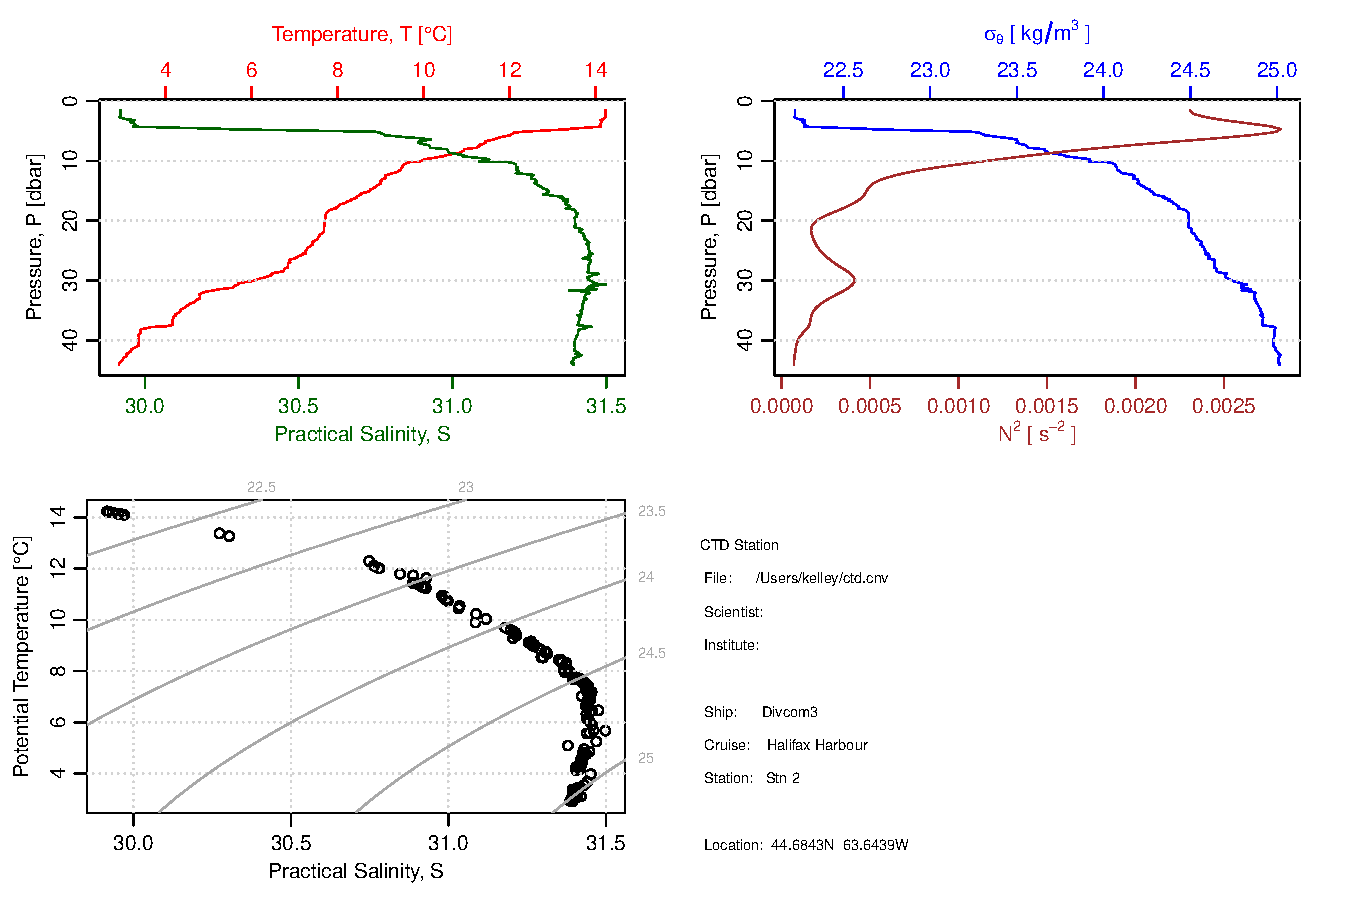
\includegraphics{oce-ctdfig}
\end{center}
\caption{Plot of CTD data with built-in dataset.}
\label{fig:ctd}
\end{figure}

The object used to hold CTD data stores not just the data, but also the raw header sequence, and
whatever has been discovered about the dataset by parsing the header; use
\begin{verbatim}
summary(ctd)
\end{verbatim}
to get a scientific overview of the data, and e.g.
\begin{verbatim}
names(ctd)
names(ctd$header)
names(ctd$data)
\end{verbatim}
to learn more about both the \verb@ctd@ object generally, and the instruments
that were attached to the CTD frame for the measurement in question.

It is also possible to plot the components individually, either by accessing the data directly
(e.g. \verb@ctd$data$pressure@ is a vector of pressure; use \verb@names(ctd)@ to discover the
names) or by using more specialized functions such as \verb@plot.TS@ and \verb@plot.profile@.
As an example of the latter,
\begin{Schunk}
\begin{Sinput}
> library(oce)
> data(ctd)
> pycnocline <- ctd.trim(ctd, "pressure", c(5, 12))
> plot.profile(pycnocline, type = "sigmatheta+N2")
\end{Sinput}
\end{Schunk}
produces Figure~\ref{fig:ctdpycnocline}. Note that the buoyancy frequency is determined by
differentiating an approximation to the density profile calculated with a smoothing cubic
spline. See the manual for \verb@N2()@ to see how to control the smoothing.
\begin{figure}
\begin{center}
\setkeys{Gin}{width=0.7\textwidth}
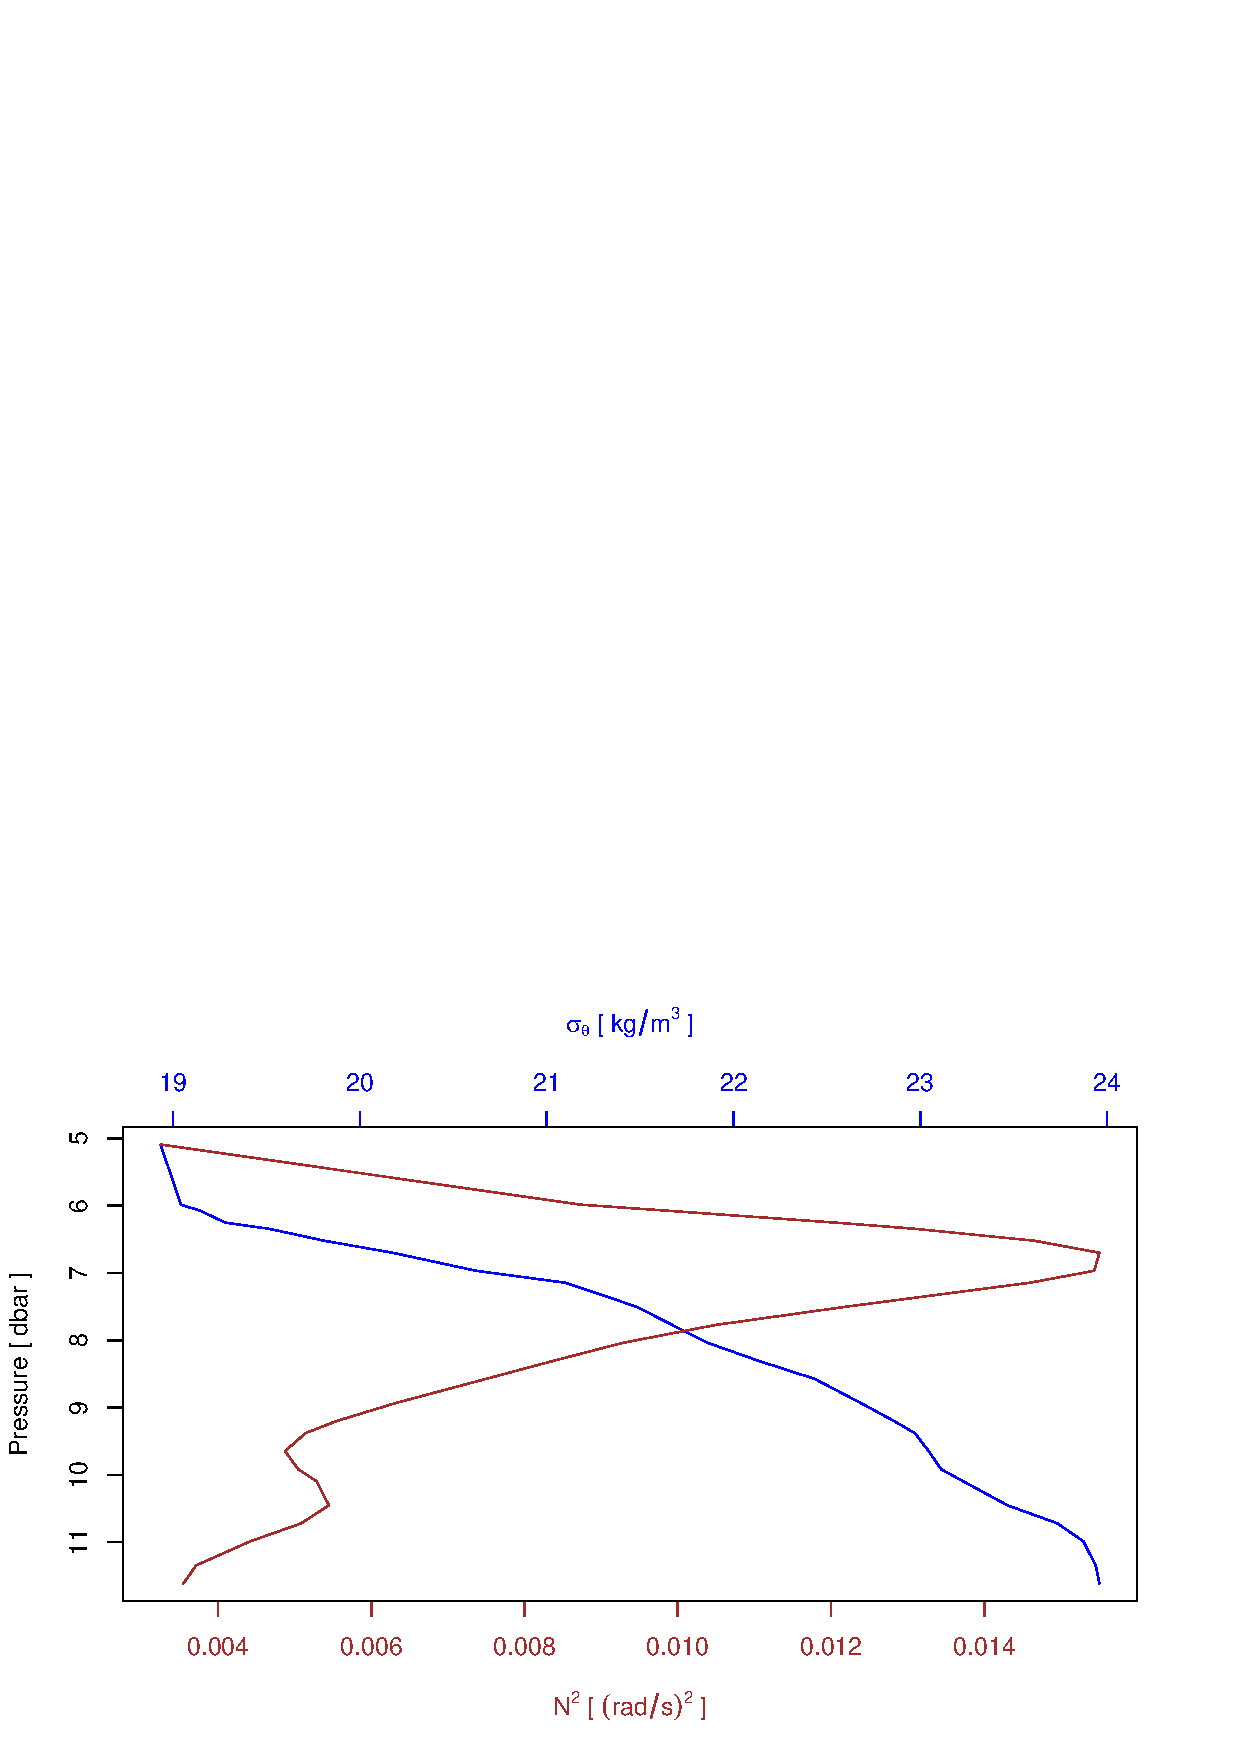
\includegraphics{oce-ctdpycnoclinefig}
\end{center}
\caption{Density and buoyancy-frequency variation within the pycnocline.}
\label{fig:ctdpycnocline}
\end{figure}


\subsection{Example with raw data}

The \verb@oce@ library provides \verb@ctd.trim()@ for trimming CTD data. It has a parameter called \verb@method@
to control the method of trimming. For quick and dirty work, \verb@method=downcast@ may be useful, but the method
is not perfect, and it is probably best to trim the data by eye. (Spending a few minutes doing this makes sense
because the data are so valuable. Do you really want your conclusions to be biased by using untrustworthy data?)

The dataset \verb@ctd.raw@ is an example of an untrimmed file.  The code
\begin{Schunk}
\begin{Sinput}
> library(oce)
> data(ctd.raw)
> plot.ctd.scan(ctd.raw)
\end{Sinput}
\end{Schunk}
\begin{figure}
\begin{center}
\setkeys{Gin}{width=\textwidth}
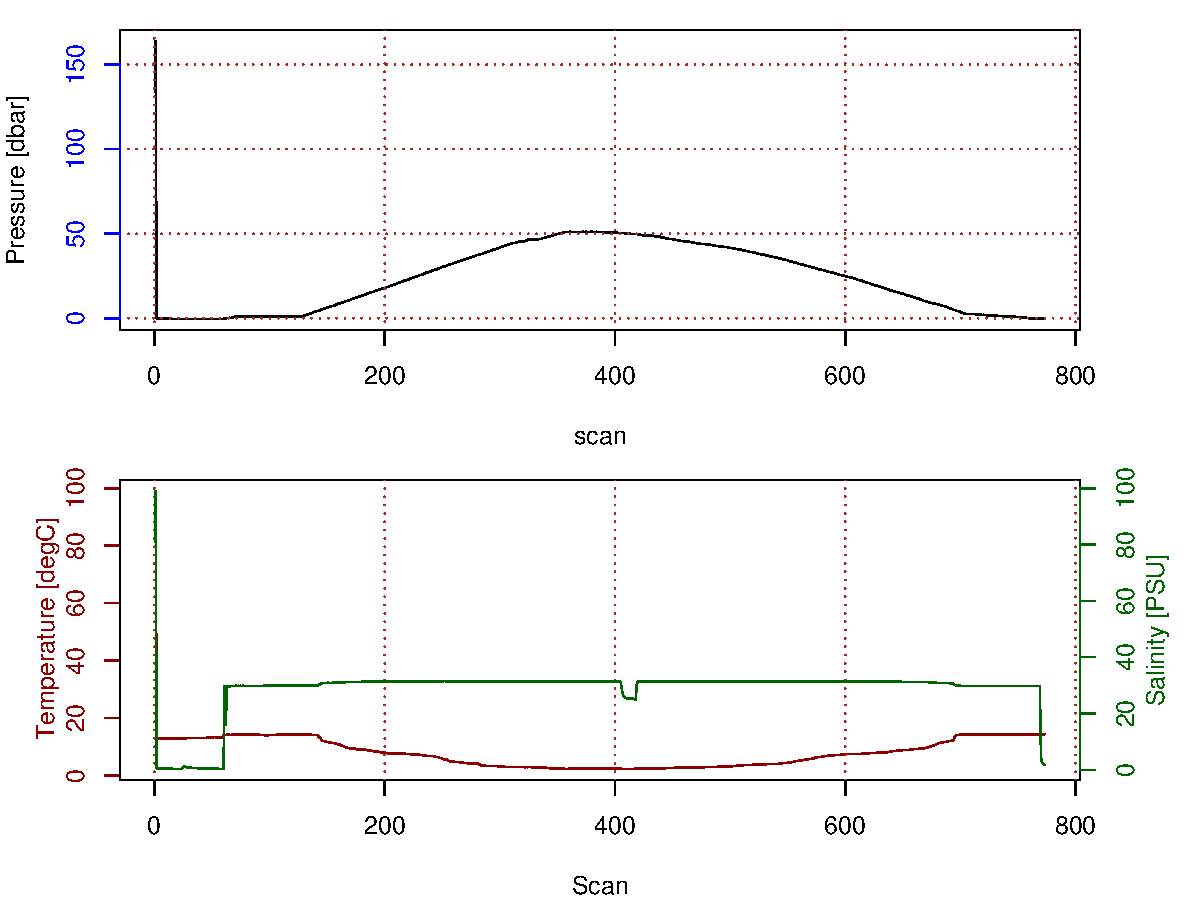
\includegraphics{oce-ctdrawfig}
\end{center}
\caption{Scanwise plot of raw CTD data.}
\label{fig:ctdraw}
\end{figure}
\noindent will create a two-panel plot (Figure~\ref{fig:ctdraw}) that is often used in the
trimming of CTD data. The bottom panel shows temperature in red and salinity in green.
Oceanographers will see in an instant that this dataset needs trimming, to isolate the downcast.  A rough trimming job can be accomplished by
\begin{verbatim}
ctd.trimmed <- ctd.trim(ctd.raw)
\end{verbatim}
and checked by
\begin{verbatim}
plot.ctd.scan(ctd.trimmed)
\end{verbatim}	
A more precise trimming job really requires an expert's eye, though.  This work
is made easy by commands such as
\begin{verbatim}
plot.ctd.scan(ctd.trim(ctd.raw, "scan", c(150,250))
\end{verbatim}
in which the numbers are altered a bit at a time.

\section{Coastline data}
The commands
\begin{Schunk}
\begin{Sinput}
> library(oce)
> data(coastline)
> plot(coastline, col = "darkred")
> hfx.lat <- 44 + 39/60
> hfx.lon <- -(63 + 34/60)
> points(hfx.lon, hfx.lat, col = "blue", cex = 3, pch = 20)
> text(hfx.lon, hfx.lat, "Halifax", col = "blue", pos = 4, cex = 1.3)
\end{Sinput}
\end{Schunk}
produce a map of the coastline of Eastern Canada (Figure~\ref{fig:coastline}). Such coastline
data are available from a variety of sources. The NOAA site
\url{http://www.ngdc.noaa.gov/mgg_coastline/}
is particularly popular, and it has the advantage
of providing data in Splus format.
\begin{figure}
\begin{center}
\setkeys{Gin}{width=0.6\textwidth}
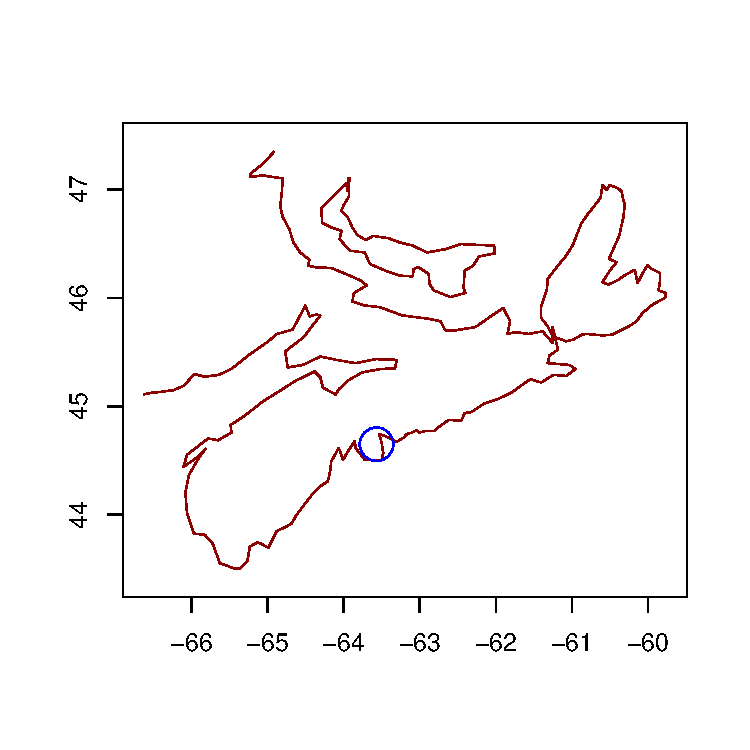
\includegraphics{oce-coastlinefig}
\end{center}
\caption{Coastline of eastern Canada, showing Prince Edward Island, New Brunswick, and Nova Scotia.  (Halifax is the home of the author.)}
\label{fig:coastline}
\end{figure}

\section{Sea-level data}

The commands
\begin{Schunk}
\begin{Sinput}
> library(oce)
> data(sealevel)
> plot(sealevel)
\end{Sinput}
\end{Schunk}
load and graph a build-in dataset of sea-level timeseries. The result, shown in
Figure~\ref{fig:sealevel}, is a four-panel plot. The top panel is a timeseries view that
provides an overview of the entire data set. The second panel is narrowed to the most recent
month, which should reveal spring-neap cycles if the tide is mixed. The third panel is a
spectrum, with a few tidal constituents indicated. At the bottom is a cumulative spectrum,
which makes these narrow-banded constituents quite visible.

\begin{figure}
\begin{center}
\setkeys{Gin}{width=\textwidth}
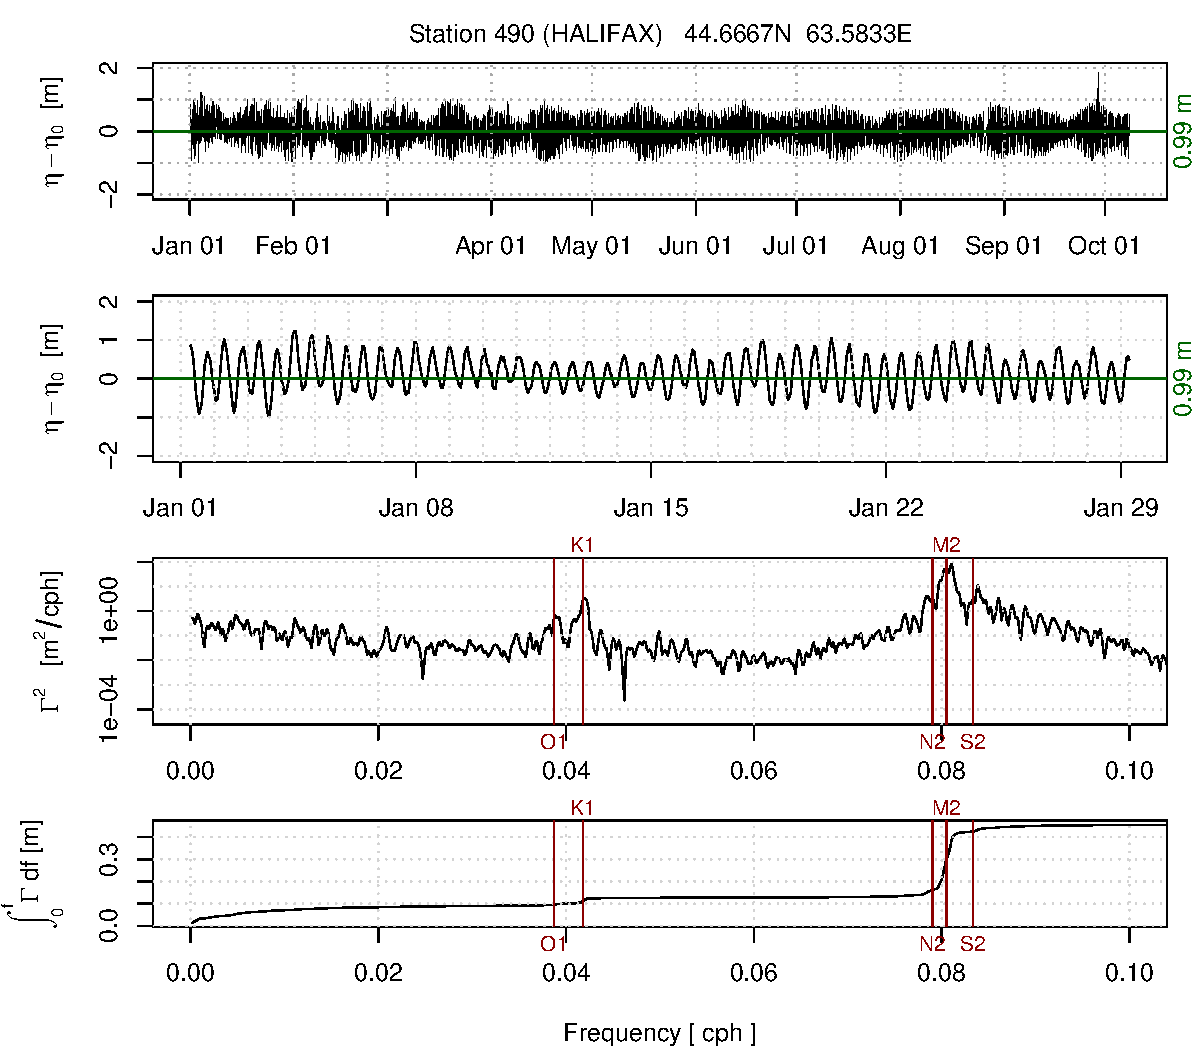
\includegraphics{oce-sealevelfig}
\end{center}
\caption{Plot of sealevel timeseries measured at Halifax, Nova Scotia.}
\label{fig:sealevel}
\end{figure}
Of course, it is possible to work directly with the data, e.g.
\begin{Schunk}
\begin{Sinput}
> spectrum(sealevel$eta, spans = 48)
> abline(v = 1/12.42)
> mtext("M2", at = 1/12.42, side = 3)
\end{Sinput}
\end{Schunk}

\section{Lobo data}
The commands
\begin{Schunk}
\begin{Sinput}
> library(oce)
> data(lobo)
> plot(lobo)
\end{Sinput}
\end{Schunk}
produce a plot (Figure~\ref{fig:lobo}) of lobo data from the Northwest Arm of Halifax Harbour.
As usual, \verb@oce@ provides access to the raw data.  Try the following, to see a TS
diagram with dots colour-coded by time:
\begin{Schunk}
\begin{Sinput}
> a <- as.numeric(lobo$time - lobo$time[1])
> hue <- 0.5 * a/max(a)
> plot.TS(as.CTD(lobo$S, lobo$T, 0), col.data = hsv(hue, 1, 1), 
+     pch = 20, cex = 2)
\end{Sinput}
\end{Schunk}
(Here, note the use of coercion to a CTD object, to get a TS diagram with density lines.)
\begin{figure}
\begin{center}
\setkeys{Gin}{width=\textwidth}
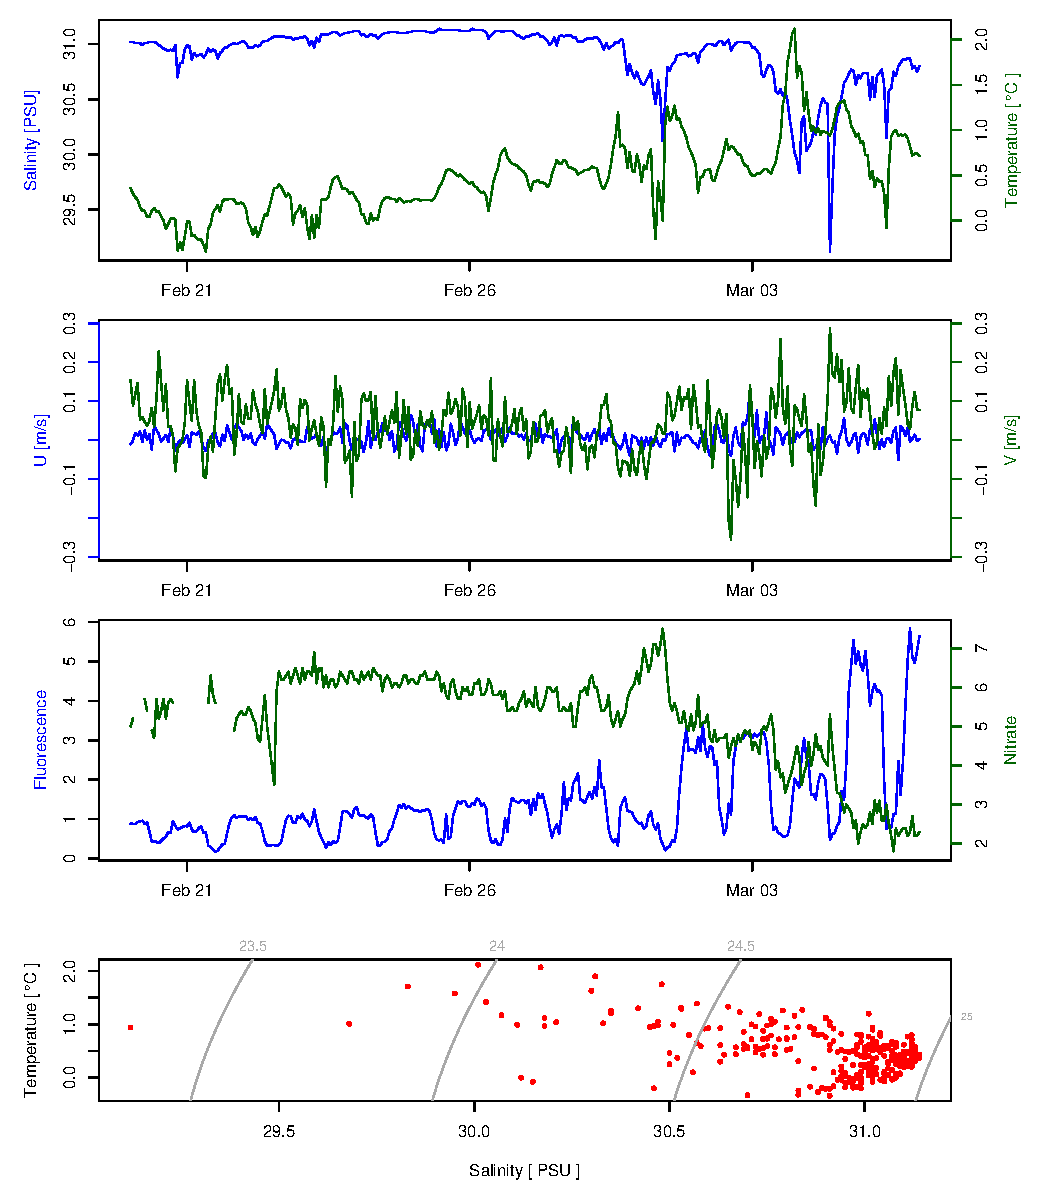
\includegraphics{oce-lobofig}
\end{center}
\caption{Plot of lobo data obtained in Northwest Arm of Halifax Harbour, just
before the Spring bloom of 2007.}
\label{fig:lobo}
\end{figure}



\section*{Appendix A: bugs}
\begin{enumerate}

\item \verb@read.lobo@ makes overly strong assumptions about which sensors will be deployed in
a LOBO instrument

\item \verb@read.ctd@ only handles data from SeaBird instruments

\end{enumerate}

\section*{Appendix B: plans}
\begin{enumerate}

\item WOCE exchange formats should be handled.

\item There should be a way to combine profile sequences into sections.

\item ADCP data should be handled.

\item Microstructure data should be handled.

\item Levitus-atlas data should be handled.

\item Air-sea flux formulae should be provided.

\end{enumerate}

\end{document}

